\section{RES task performance}

\section{Mutation generation}

\subsection{Design choice: discarding wrongly predicted position}

\subsection{Design choice: experimental vs AlphaFold structures}

\section{Protein fitness prediction}


\begin{table}[!t]
\caption{Average performance on generating better than wildtype mutations of our models. We also include statistics for the Tranception model. Numbers in \textbf{bold} represent the highest score per column, while numbers with an \underline{underline} represent the second highest score per column.}
\label{generation-results}
\vskip 0.15in
\begin{center}
\begin{scriptsize}
\begin{sc}
\begin{tabular}{@{}ccccccc@{}}
\toprule
\multirow{2}{*}{Model} & \multirow{2}{*}{Ranking strategy} & \multicolumn{3}{c}{Spearman's rank correlation} & \multirow{2}{*}{\begin{tabular}[c]{@{}c@{}}Top 10\\ precision\end{tabular}} & \multirow{2}{*}{\begin{tabular}[c]{@{}c@{}}Top 10\\ recall\end{tabular}} \\ \cmidrule(lr){3-5}
                       &                                   & Average    & Worse than WT   & Better than WT   &                                                                             &                                                                          \\ \midrule
EQGAT                  & Positional                        & 0.223      & 0.128           & 0.118            & 0.486                                                                       & \underline{0.187}                                                                    \\
EQGAT                  & Global                            & \underline{0.262}      & \underline{0.154}           & \underline{0.157}            & \underline{0.491}                                                                       & 0.072                                                                    \\
GVP                    & Positional                        & 0.106      & $-0.009$          & \textbf{0.276}            & 0.462                                                                       & \textbf{0.419}                                                                    \\
GVP                    & Global                            & 0.202      & 0.128           & $-0.011$           & 0.426                                                                       & 0.100                                                                    \\
TRANCEPTION            &                                   & \textbf{0.429}      & \textbf{0.299}           & 0.143            & \textbf{0.619}                                                                       & 0.012                                                                    \\ \bottomrule
\end{tabular}
\end{sc}
\end{scriptsize}
\end{center}
\vskip -0.1in
\end{table}


\begin{figure}
    \centering
    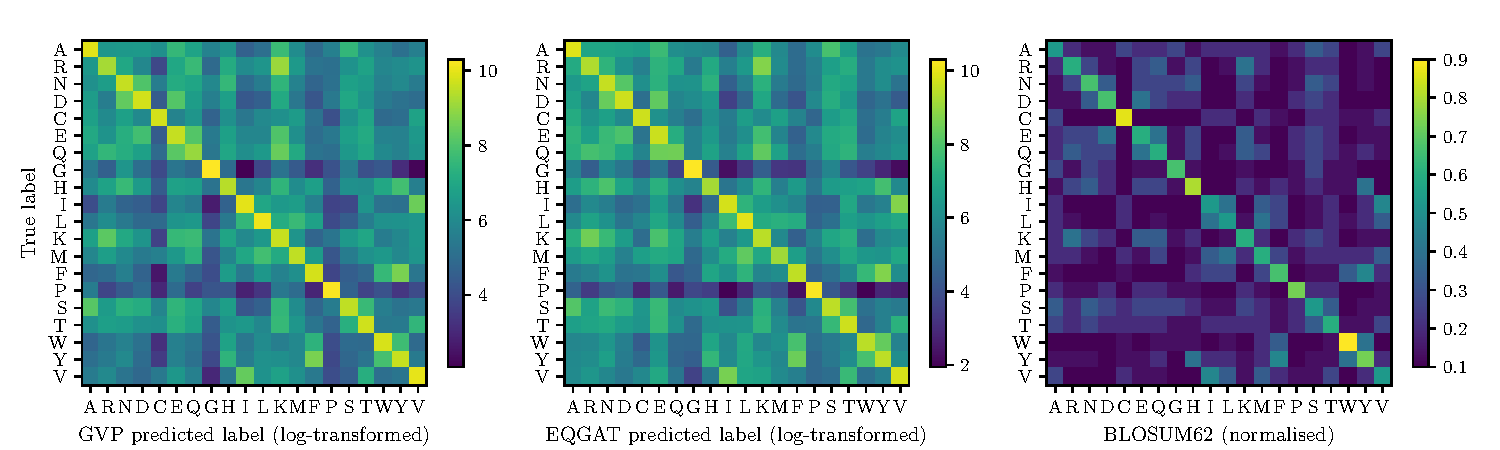
\includegraphics[width=\textwidth]{masters-report/figures/confusion_matrices.pdf}
    \caption{Comparison between the confusion matrices of EQGAT and GVP to the BLOSUM62 matrix.}
    \label{fig:confusions}
\end{figure}
